\section{Implementation}
\label{sec:streamimplementation}

\subsection{Abstractions choice}

As stated in the Architecture part, a stream processor is composed of one Iteratee in input of N Enumerators in output (one per child). Distribution is done using HTTP stream on top of TCP. Custom processors on top of Iteratees have been selected over actors for several reasons.

First, actors does not handle back-pressure in a built-in way. But back-pressure is very important for our system in order to optimize the resources used. Back-pressure is even
used from a parent's local journal to its children using the reactive MongoDB driver ReactiveMongo \footfullcite{bib:reactivemongo} that exposes methods returning Iteratee / Enumerators. It is really
convenient to have only one composable abstraction to compose streams with back-pressure from MongoDB or from other processors. 

Moreover, actors does not have a simple mechanism to sequentially compose asynchronous operations. When an actor processes a message and call an asynchronous function (which
returns a Future), it handle the next message in its mailbox meanwhile. An actor cannot "block in a non-blocking way" over asynchronous operations as Iteratees can. There exists
a solution using the Stash trait \footfullcite{bib:stashtrait} that allows to put in local memory the messages that we want to process after the current event has been asynchronously processed, but it is not fault-tolerant if the actor fails and not efficient as messages are swapped between the mailbox and the actor local memory (and not compatible with back-pressure).

In the end, Iteratees, Futures and Promises are better abstractions than actors to handle this problem.

\subsection{PathId serialization and deserialization into MongoDB}

The PathId Scala class is composed of the MongoDB id of the root event inserted in the Journal, plus a Vector of Int that represents the Path in the generational event tree.
A MongoDB id is an id created by the Scala MongoDB driver that is a 24-char hexadecimal string made with the current time plus a local incremental counter in order to guarantee that
each document id is unique and that the id of events are strictly ascendant to retain the order of insertion.

By default, MongoDB uses the \_id field of a document to put an unique id. Moreover, all MongoDB's collections have a default index on this field. Thus,
for simplicity and efficiency, we will serialize PathId to a hexadecimal string to put as a value of this \_id field. This serialization has to maintain the order
of events in a local journal. Indeed, ReactiveMongo's stream capabilities from MongoDB allows to get from MongoDB a stream of all the documents of a collection since a particular id. Therefore, this id has to be ascendant for all events of a local journal (to define the order, MongoDB does a simple String comparison from left to right).

The simple way to do this is to first put the root event 24-char id, and then put each integer of the path id on a padded 8-char byte. The padding allows easy deserialization.

With this serialization, events that are the same height in the tree have ids with the same number of chars (so in particular, all event ids generated by a processor have the same size). Moreover, locally in each local journal of processor, all events generated from a root event 01 created before root event 02 will have an id smaller than all events
generated from root event 02 (because they have the same size, and the root event id 01 has a higher id than 02 which are at the left of the serialized PathId). Furthermore,
sibling nodes in the event tree have an incremental number according to their creation order, so order is ensured in a substream. Figure \ref{fig:pathidserde} illustrates this serialization and ordering mechanism. With this model, for each input event, a processor can generate sub-events with an additional 4-byte part at the end of the PathId, so
for each event a processor can generate at maximum 2 power 32 events (around 4 billion events).

\begin{figure}[h]
  \begin{center} 
    \makebox[\textwidth]{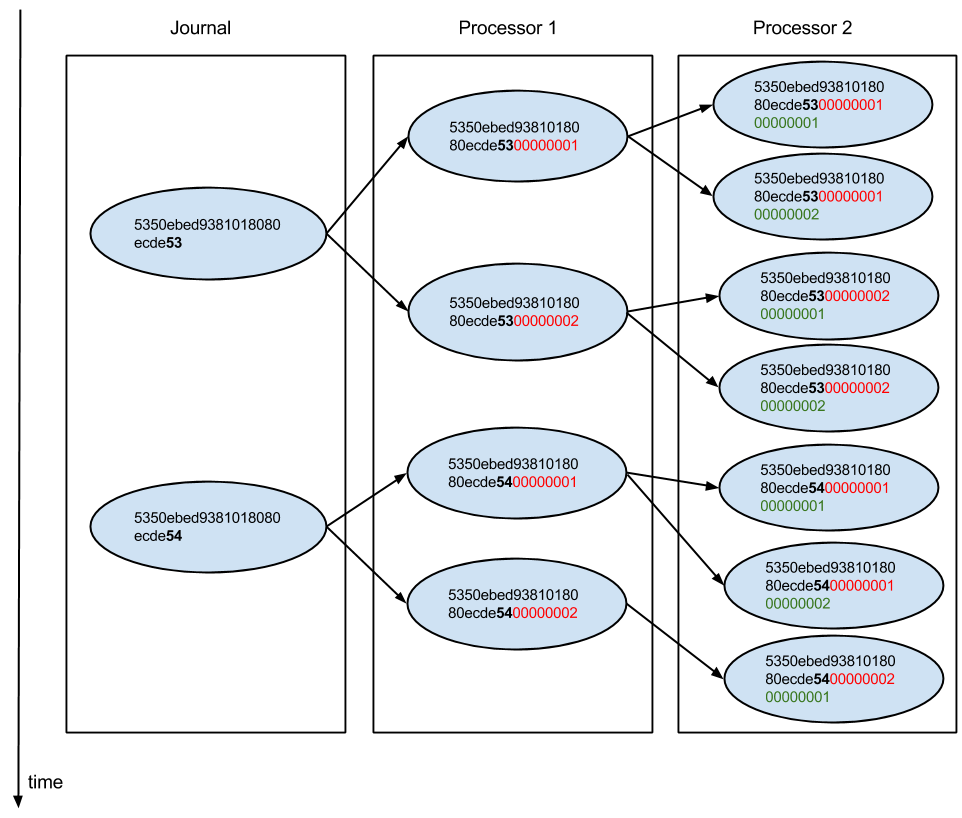
\includegraphics[width=1.0\textwidth]{img/pathidserde.png}}
    \caption{PathId serialization ensuring ordering in MongoDB local journals}
    \label{fig:pathidserde}
  \end{center}
\end{figure}

Listing \ref{lst:pathidserde} shows the code of Path Id and its serialization and deserialization.

\begin{listing}[h]
\begin{minted}[fontsize=\codesize, frame=lines, framesep=2mm]{scala}
case class PathId(rootEvent: String, path: Vector[Int])

object PathId {
  import reactivemongo.bson.utils.Converters
  import java.nio.ByteBuffer

  def apply(rootEvent: String): PathId = PathId(rootEvent, Vector.empty)

  def serialize(id: PathId): String = {
    val array = id.path
    val byteBuffer = ByteBuffer.allocate(array.length * 4)
    val intBuffer = byteBuffer.asIntBuffer
    intBuffer.put(array.toArray)
    byteBuffer.flip()

    id.rootEvent + Converters.hex2Str(byteBuffer.array())
  }

  def deserialize(str: String): PathId = {
    val (idStr, pathStr) = str.splitAt(12*2)

    val byteBuffer = ByteBuffer.allocate(4)
    val arrayBytes = Converters.str2Hex(pathStr)
    val path = arrayBytes.grouped(4).toVector map { bytes =>
      byteBuffer.put(bytes)
      byteBuffer.flip()
      val int = byteBuffer.getInt
      byteBuffer.clear()
      int
    }

    PathId(idStr, path)
  }

  val min = PathId("000000000000000000000000")
}
\end{minted}
\caption{PathId serialization and deserialization}
\label{lst:pathidserde}
\end{listing}


\subsection{Stream processors}

A stream processor is composed of one Iteratee in input of N Enumerators in output (one per child). 
In order to link the Iteratee with the Enumerators, we use Promise to be able to complete manually a Future, and Scala STM to handle concurrent access. 

When the Iteratee receives an input event, it processes it to create a substream that is flattened into the main stream using the Enumeratee.mapFlatten helper. Moreover, the Enumeratee updatePathId is responsible of updating the PathId of each sub-event with the new level in the event tree.

Then, each sub-event goes through the effector method that is an Enumeratee executing asynchronously and sequentially the performAtomicSideEffect method (that is the insertion
in the local journal for persistent processors). 

Last, sub-events go in the downstreamTrigger Iteratee that update the state of each child according to the state transition diagram Figure \ref{fig:childstates}. Moreover, each
child that is UpToDate had previously registered a Promise to trigger in the consumersTrigger Map. This promise is linked to a Future that is returned by the Enumerator of a child
when this one is up to date. Thus, when we call promise.trySuccess(Some(outEvent)), the Future pushed in the Enumerator is fulfilled with the new sub-event (and so it will be sent
to the child).
\\

In the Enumerator corresponding to a child (the createOutStream method), when the code is called a new time (corresponding the ACK that previous events has been processed by the child in local mode,
or that the events are at least in the TCP send buffer in distributed mode), we check the state of the child. If it is UpToDate or WaitingForDownStreamAck, we register
a promise to be called when a new event will come in, and we put the Future linked to the promise into the Enumerator. This mechanism allows non-blocking long-polling.
If it is Late, we call the since method the retrieve the past events from the sinceId parameter. If the processor is a persistent stream processor,
it will directly take the past event streams from its MongoDB local journal and returns an Enumerator of it using the ReactiveMongo reactive driver. If the processor is
a side-effect stream processor, it will ask its parent for the past event streams, removing the last node of the path id and then filtering the substream via an offset (as explained in the architecture part). 

Figure \ref{fig:createOutStream} illustrates this mechanism. Listing \ref{lst:processor} shows the code of the generic stream processor. Listing \ref{lst:psprocessor} shows the code of persistent stream processor and side-effect stream processor. 

\subsection{Journal}















